One way to decrease the time complexity is the elimination of repeated calculations. The main idea is simple: do the computation once and save the result for later.
There are several versions of this approach; we define the \textbf{variable elimination} algorithm. \vspace{3.5pt}

Variable elimination works by evaluating expressions in \textbf{right-to-left} order. Intermediate results are stored, and summations over each variable are done only for 
those portions of the expression that depend on the variable. By this algorithm the equation becomes:
\begin{itemize}
    \renewcommand{\labelitemi}{}
    \item $\mathbf{P}(B|j, m)$
    \item $= \alpha P(B) \sum_{e} P(e) \sum_{a} P(a|B, e) P(j, a) P(m, a)$
    \item $= \alpha f_B(B) \sum_{e} f_E(e) \sum_{a} f_A(b, e) f_J(a) f_M(a)$
\end{itemize}
Each part of the expression was annotated with the name of the corresponding \textbf{factor}; a factor is a matrix containing values of its argument variables.
For instance, the factor $f_J(a)$ correspond to $P(j|a)$, and it's a two-element vector containing the same values of the CPT.
\begin{center}
    $f_J(a) = 
        \begin{bmatrix}
            P(j|a) \\ 
            P(j|\neg a) \\ 
        \end{bmatrix}
    = 
        \begin{bmatrix}
            0.90 \\ 
            0.05 \\ 
        \end{bmatrix}
    $
\end{center}
Even if factors are matrix like representation, the product between two or more of them is not the ordinary matrix multiplication but instead the \textbf{pointwise product} operation.
The process of evaluation is a process of \textbf{summing out} variables, composed by two main steps:
\begin{itemize}
    \renewcommand{\labelitemi}{-}
    \item Move any constant factors outside the summations, as happens for the prior probabilities.
    \item Add up submatrices in pointwise product of remaining factors, creating new factors.
\end{itemize}
Let's see an example for better understanding.
\begin{example}
    i.e. $JohnCalls$, $MaryCalls$ and $Alarm$ CPTs. \vspace{3.5pt}

    \begin{center}
        \includegraphics[width=0.6\textwidth]{img/img13.png}
    \end{center} \vspace{3.5pt}

    We just said that each CPTs can be written as a factor - a matrix like representation contaning the same values of the conditional probability. \vspace{3.5pt}

    We are going to sum out $A$ from the product of $f_A$, $f_J$ and $f_M$. Before summing out A, we have to solve the pointwise product of the same factors. \vspace{3.5pt}

    \begin{itemize}
        \renewcommand{\labelitemi}{}
        \item $\mathbf{P}(B|j,m)$
        \item $= \alpha \mathbf{P}(B|j, m)$
        \item $= \alpha P(b)\sum_{e}P(e)\sum_{a}P(e)P(a|e, b)P(j|a)P(m|a)$
        \item $= \alpha f_B(B) \sum_{e} f_E(e) \sum_{a} f_A(b, e) f_J(a) f_M(a)$
        \item $= \alpha f_B(B) \sum_{e} f_E(e) \sum_{a} f_{AJM}(b, e, a)$
        \item $= \alpha f_B(B) \sum_{e} f_E(e) f_{\overline{A}JM}(b, e)$
        \item 
        \item $\mathbf{P}(B|j,m) = \alpha f_B(B) \sum_{e} f_E(e) f_{\overline{A}JM}(b, e)$
    \end{itemize} \vspace{7pt}
    Examing this sequence, we see that the two computational operations are performed: initially we define for each conditional probability its corresponding factor,
    then we compute the pointwise product of $f_A$, $f_J$ and $f_M$ (\textit{as shown in the fourth passage}) and finally we sum out $A$ from the new factor ($f_{\overline{A}JM}(b, e)$)
    created. \vspace{7pt}

    In the end we repeat the same process summing out $E$.
    \begin{itemize}
        \renewcommand{\labelitemi}{}
        \item $\mathbf{P}(B|j,m)$
        \item $= \alpha f_B(B) \sum_{e} f_E(e) f_{\overline{A}JM}(b, e)$
        \item $= \alpha f_B(B) \sum_{e} f_{\overline{A}JME}(b, e)$
        \item $= \alpha f_B(B) f_{\overline{AE}JM}(b)$
    \end{itemize}
\end{example}
Before starting the computation, it would be a good idea to remove all irrelevant random variables. According to this last observation,
there are some theorems that can help us achieve our goal.
\begin{definition}[title={Theorem}]
    Y is \textbf{irrelevant} unless $Y \in Ancestors({X} \cup \mathbf{E})$
\end{definition}
\begin{definition}[title={Theorem}]
    Y is \textbf{irrelevant} if \textit{d-separated} from $\{X\}$ by $\mathbf{E}$
\end{definition}
\begin{example}
    i.e. Application of previous theorems. \vspace{3.5pt}
    \begin{center}
        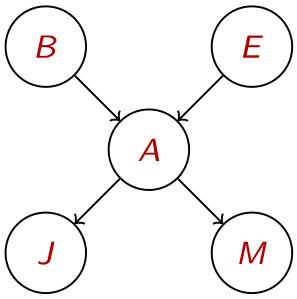
\includegraphics[width=0.3\textwidth]{img/img14.png}
    \end{center} \vspace{3.5pt}

    Let's consider the following simple query: \vspace{3.5pt}
    \begin{center}
        $P(JohnCalls|Burglary = true)$
    \end{center} \vspace{3.5pt}
    So, which is the probability of $JohnCalls$ given $Burglary$ true? The solution of this kind of query can be written as products of conditional probabilities, such as: \vspace{7pt}
    \begin{itemize}
        \renewcommand{\labelitemi}{}
        \item $P(JohnCalls|Burglary = true)$
        \item $= \alpha P(b) \sum_{e}P(e) \sum_{a}P(a) P(a|b,e) P(j|a) P(m|a)$
    \end{itemize} \vspace{3.5pt}
    As you can assume, we have already moved out probabilities ($P(b)$, $P(e)$) that do not belong in the summations. By the way, also another observation we can do: node $MaryCalls$
    does not belong to $JohnCalls$'s Ancestors. Therefore, $MaryCalls$ conditional probability should not be considered inside the equation; Ancestors' theorem help us to simplify the
    final expression. In probabilistic terms these assertions are defined as: \vspace{3.5pt}
    \begin{itemize}
        \renewcommand{\labelitemi}{}
        \item $X = JohnCalls$ , $\mathbf{E}=\{Burglary\}$
        \item $Ancestors(\{X\} \cup \mathbf{E}) = \{Alarm, Earthquake\}$ so $MaryCalls$ is \textbf{irrelevant}.
    \end{itemize} \vspace{3.5pt}
    \begin{center}
        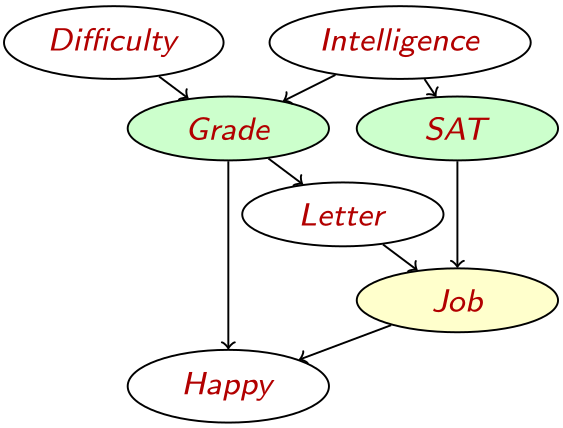
\includegraphics[width=0.4\textwidth]{img/img15.png}
    \end{center} \vspace{3.5pt}

    Now we switch to the student network, the new simple query is:
    \begin{center}
        $P(Job|Grade, SAT) = ?$
    \end{center} \vspace{3.5pt}
    The second theorem uses the notion of \textit{d-separation}. It could be convenient to pick up on its main concept: \vspace{3.5pt}
    \begin{center}
        The nodes $X$ and $Y$ are \textit{d-separated} given $Z$ if there is no \textit{active trail} between $X$ and $Y$ given $Z$. $Z$ cannot be part of the active trail.
    \end{center} \vspace{3.5pt}
    For $P(Job|Grade, SAT)$, not only $Happy$ is irrelevant, it does not belong to $Ancestors(\{Job\} \cup Grade, SAT)$, but also $Difficulty$ and $Intelligence$ are \textit{d-separated}
    from $Job$, given $Grade$ and $SAT$. Accordingly, $Happy$, $Difficulty$ and $Intelligence$ should not be considered in the simple query.
\end{example}